% !TEX program = xelatex
% RMA RSS 2021: main pp. 4-6, Fig. 2; supplement Algorithms 1-2.
% Original imagegen draft retained unchanged through graphicx viewports.
% Illustration + vector typography/arrows; not an all-vector illustration.
\documentclass[tikz,border=2mm]{standalone}
\usepackage{fontspec,xeCJK,amsmath,amssymb,graphicx,lmodern}
\setsansfont{Arial}
\setCJKmainfont[Path=/System/Library/Fonts/,BoldFont={STHeiti Medium.ttc}]{STHeiti Light.ttc}
\setCJKsansfont[Path=/System/Library/Fonts/,BoldFont={STHeiti Medium.ttc}]{STHeiti Light.ttc}
\renewcommand{\familydefault}{\sfdefault}
\usetikzlibrary{arrows.meta,calc}
\definecolor{ink}{HTML}{172D40}
\definecolor{muted}{HTML}{526674}
\definecolor{warm}{HTML}{BC5B28}
\definecolor{warmbg}{HTML}{FFF7ED}
\definecolor{teal}{HTML}{087E87}
\definecolor{tealbg}{HTML}{F0FAFA}
\definecolor{blue}{HTML}{237DB1}
\definecolor{bluebg}{HTML}{F1F8FD}
\tikzset{txt/.style={text=ink,font=\fontsize{15}{18}\selectfont,align=center,inner sep=1pt},
 sm/.style={txt,font=\fontsize{12}{15}\selectfont},
 hd/.style={txt,font=\bfseries\fontsize{20}{23}\selectfont},
 ar/.style={-{Stealth[length=2.5mm]},draw=ink,line width=1.2pt,rounded corners=3pt},
 sup/.style={ar,draw=warm,dashed},
 box/.style={rounded corners=5pt,line width=.8pt,draw=teal!55,fill=white}}
\newcommand{\textat}[4]{\node[txt,text width=#3*.3mm]at(#1,#2){#4};}
\newcommand{\smallat}[4]{\node[sm,text width=#3*.3mm]at(#1,#2){#4};}
\newcommand{\headat}[4]{\node[hd,text width=#3*.3mm]at(#1,#2){#4};}
\newcommand{\art}[7]{\begingroup
 \pgfmathsetmacro{\bt}{1536-#2-#4}\pgfmathsetmacro{\rt}{1024-#1-#3}
 \pgfmathsetlengthmacro{\aw}{#7*.3mm}
 \node[anchor=north west,inner sep=0,outer sep=0]at(#5,#6){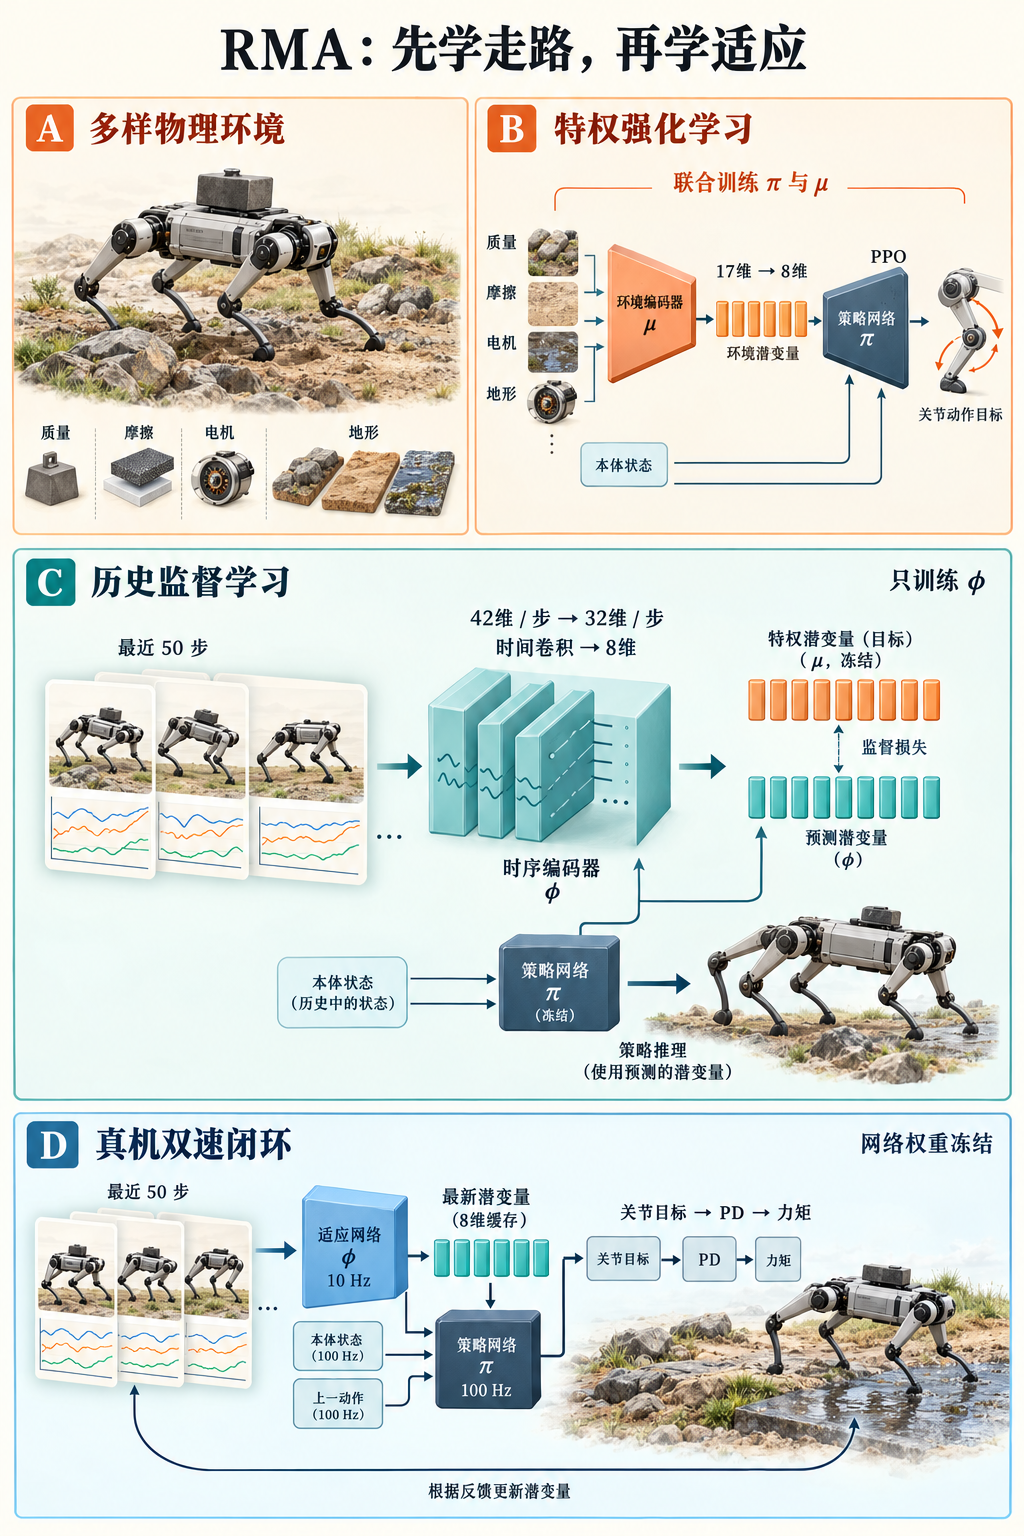
\includegraphics[trim=#1bp \bt bp \rt bp #2bp,clip,width=\aw]{rma-imagegen-draft.png}};
\endgroup}
\newcommand{\tok}[3]{\foreach \i in {0,...,7}{\filldraw[fill=#3!35,draw=#3,rounded corners=1pt]({#1+\i*13},#2)rectangle++(9,25);}}
\begin{document}
\begin{tikzpicture}[x=.3mm,y=-.3mm]
\path[use as bounding box](0,0)rectangle(1050,1455);
\fill[white](0,0)rectangle(1050,1455);
\headat{525}{32}{1020}{RMA：先学会走，再从反馈中判断怎么走}
\textat{525}{68}{1020}{训练分两阶段；部署时改潜变量，网络权重固定}

% A: physical context with complete retained robot illustration.
\draw[box,draw=warm!50,fill=warmbg](12,98)rectangle(335,450);
\headat{174}{124}{300}{A\quad 多样物理环境}
\art{18}{164}{443}{248}{24}{155}{300}
\smallat{174}{348}{300}{不平地面、载荷、摩擦、电机强度}
\textat{174}{385}{295}{特权环境量 $e_t\in\mathbb R^{17}$}
\smallat{174}{425}{296}{仿真知道；真机部署不读取}

% B: policy/encoder learned jointly, exact dimensions.
\draw[box,draw=warm!50,fill=warmbg](348,98)rectangle(1038,450);
\headat{690}{124}{660}{B\quad 第一阶段：特权强化学习}
\art{609}{243}{89}{141}{468}{170}{86}
\shade[left color=ink!70,right color=ink,draw=ink](757,190)--(839,175)--(839,292)--(757,277)--cycle;
\textat{797}{234}{75}{\color{white}策略\\$\pi$}
\textat{400}{235}{90}{$e_t$}
\draw[ar](432,235)--(464,235);
\tok{602}{222}{warm}
\draw[ar](557,235)--(598,235);
\draw[ar](709,235)--(750,235);
\draw[ar](844,235)--(890,235);
\textat{951}{233}{155}{$a_t\in\mathbb R^{12}$\\目标关节角}
\smallat{510}{316}{210}{$\mu$: $17\to256\to128\to8$}
\textat{655}{274}{180}{$z_t=\mu(e_t)$}
\smallat{795}{316}{150}{$\pi$: 隐层 128}
\textat{676}{363}{620}{$a_t=\pi(x_t,a_{t-1},z_t)$，输入 $30+12+8=50$ 维}
% The policy equation explicitly names current state and previous action inputs.
\smallat{690}{417}{650}{环境反馈奖励 $r_t$；PPO 联合更新 $\pi$ 与 $\mu$\\前进奖励 + 能耗、冲击、平滑等惩罚；惩罚由弱变强}

% C: adaptation training with on-policy trajectories and frozen teacher.
\draw[box,draw=teal!50,fill=tealbg](12,465)rectangle(1038,939);
\headat{525}{493}{1010}{C\quad 第二阶段：从动作与响应中估计潜变量}
\art{36}{671}{333}{216}{29}{546}{255}
\art{426}{671}{244}{184}{391}{557}{202}
\smallat{154}{746}{270}{最近 50 步，约 0.5 秒\\每步：本体状态 + 已执行动作}
\textat{487}{750}{300}{每步 $42\to32$ 维\\三层时间卷积 $\to8$ 维}
\draw[ar](288,635)--(381,635);
\smallat{333}{605}{96}{历史输入}
\draw[ar](598,635)--(646,635);
\tok{660}{624}{teal}
\textat{714}{682}{160}{$\hat z_t=\phi(H_t)$}
\textat{887}{549}{267}{$z_t=\mu(e_t)$，$\mu$ 固定}
\tok{835}{584}{warm}
\draw[sup](886,615)--(886,675);
\draw[ar](770,638)-|(823,691);
\draw[box,draw=warm!65,fill=warmbg](813,676)rectangle(1014,754);
\textat{913}{714}{195}{$\mathcal L_\phi=\|\hat z_t-z_t\|_2^2$}
\smallat{904}{786}{240}{监督目标来自特权编码\\只更新 $\phi$ 的参数}
\draw[box](40,817)rectangle(775,917);
\textat{408}{842}{720}{采样时也用预测的 $\hat z_t$ 驱动固定策略 $\pi$}
\smallat{408}{884}{710}{估计有误的行走 → 新历史 $H_t$ → 监督训练 → 再次采样\\让适应器见到自身误差造成的偏离，而非只看完美步态}
\smallat{900}{873}{220}{实线：计算 / 数据\\虚线：监督目标}

% D: deployment dataflow, never a parameter update.
\draw[box,draw=blue!50,fill=bluebg](12,955)rectangle(1038,1418);
\headat{525}{983}{1010}{D\quad 真机双速闭环：慢判断，快出动作}
\art{36}{671}{333}{216}{31}{1051}{196}
\smallat{126}{1194}{205}{状态、动作历史 $H_t$\\图中卡片为行走示意}
\draw[box,draw=blue](275,1066)rectangle(445,1144);
\textat{360}{1105}{165}{$\phi$：10 Hz\\更新 $\hat z$}
\draw[ar](232,1105)--(270,1105);
\tok{503}{1092}{teal}
\draw[ar](449,1105)--(497,1105);
\smallat{556}{1056}{185}{缓存最新 8 维 $\hat z$}
\draw[ar](556,1124)--(556,1186);
\draw[box,draw=blue,fill=white](455,1190)rectangle(656,1275);
\textat{556}{1232}{195}{$\pi$：100 Hz\\读取最新 $\hat z$}
\draw[box,draw=blue](261,1208)rectangle(414,1264);
\textat{337}{1235}{148}{$x_t,\ a_{t-1}$}
\draw[ar](418,1235)--(450,1235);
\draw[ar](660,1235)--(700,1235);
\draw[box,draw=blue](704,1205)rectangle(797,1263);
\textat{751}{1235}{88}{PD}
\smallat{726}{1178}{130}{$a_t$ 关节目标}
\art{704}{910}{294}{153}{807}{1174}{217}
\draw[ar](801,1235)--(823,1235);
\smallat{922}{1313}{215}{力矩作用于机器人\\新的本体反馈回写历史}
\draw[ar](920,1346)--(920,1375)--(126,1375)--(126,1232);
\smallat{496}{1344}{520}{$\tau_t=55(a_t-q_t)-0.8\dot q_t$，目标关节速度为 0}
\smallat{525}{1400}{990}{部署不读取 $e_t$，不运行 $\mu$，不做梯度更新；策略无需等待适应器同步}
\smallat{525}{1440}{1020}{$x_t\in\mathbb R^{30}$：12 角度 + 12 角速度 + 2 姿态角 + 4 足接触；$H_t$ 为最近 50 步历史}
\end{tikzpicture}
\end{document}
